\chapter{Additional Results}
\label{chapter:appendix_results}

%%%%%%%%%%%%%%%%%%%%%%%%%%%%%%%%%%%%%%%%%%%%%%%%%%%%%%%%%%%%%%%%%%%%%%%%%%%%%%%%%%%%%

\begin{figure}[bt]
    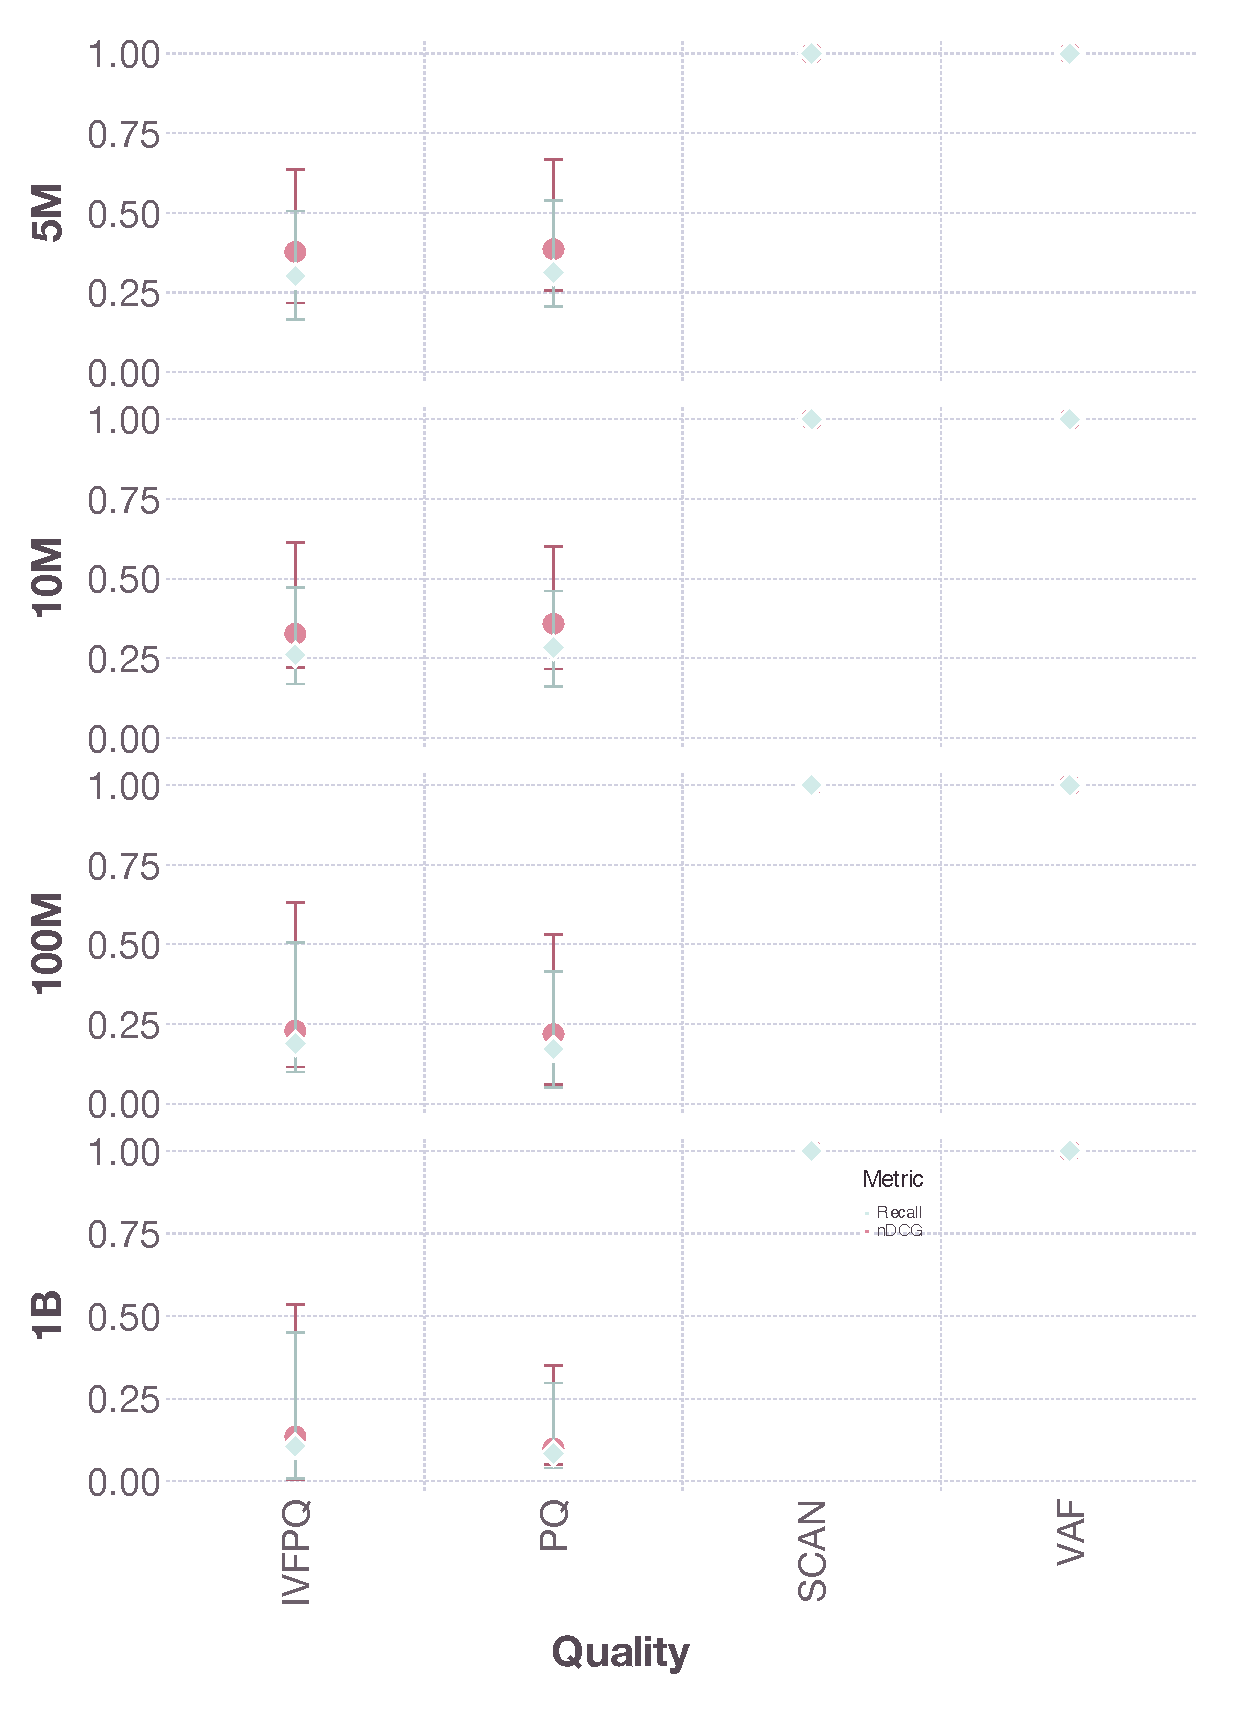
\includegraphics[width=\linewidth]{figures/bignns-cottontail-quality-NNS}
    \caption{Quality metrics for Cottontail DB during the simple \acrshort{nns} large-scale retrieval evaluation presented in \Cref{section:evaluation_bignns_cottontail}. Recall and \acrshort{dcg} are 1.0 for all execution strategies other than \acrshort{pq}, for which they exhibit rather low values with a large spread.}
    \label{figure:appendix_bignns_cottontail_nns_quality}
\end{figure}

\begin{figure}[bt]
    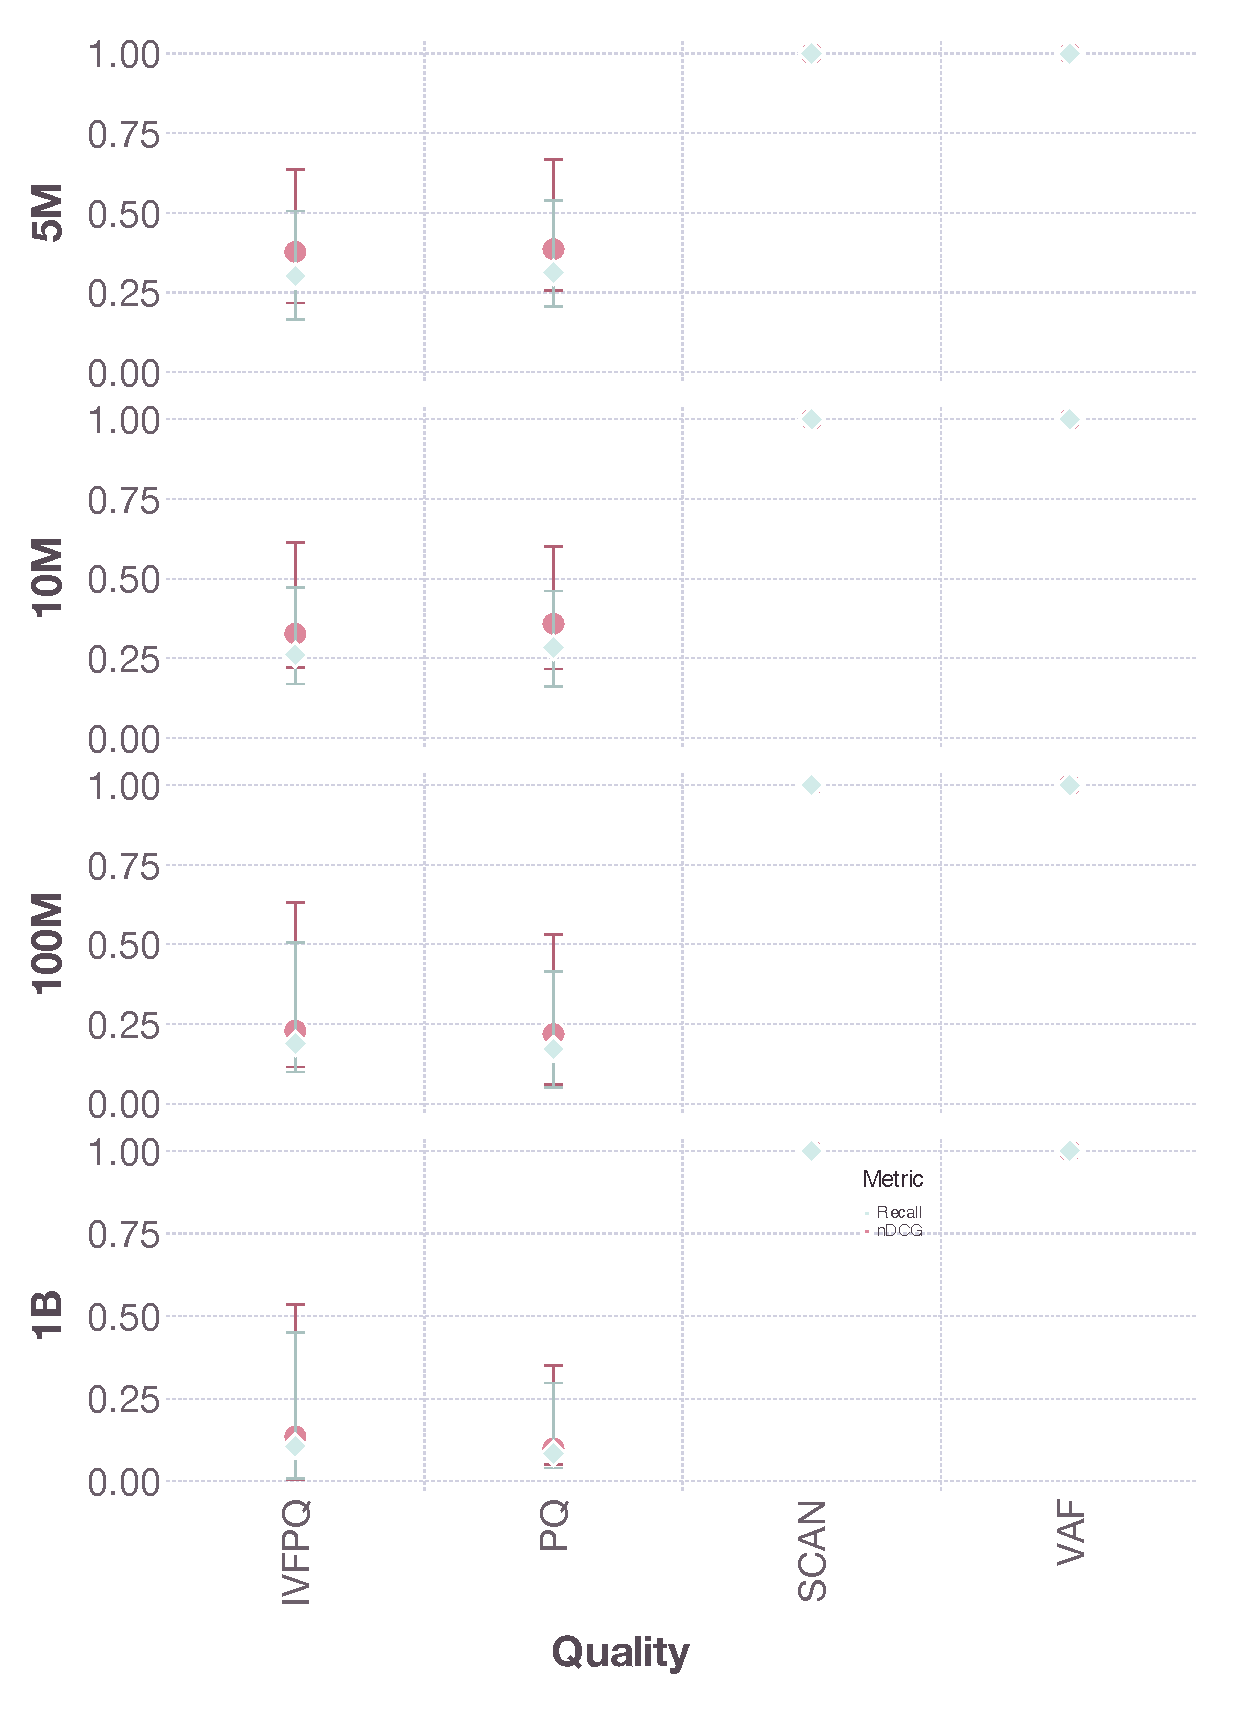
\includegraphics[width=\linewidth]{figures/bignns-cottontail-quality-NNS + Fetch}
    \caption{Quality metrics for Cottontail DB during the \acrshort{nns} + fetch large-scale retrieval evaluation presented in \Cref{section:evaluation_bignns_cottontail}. Recall and \acrshort{dcg} are 1.0 for all execution strategies other than \acrshort{pq}, for which they exhibit rather low values with a large spread.}
    \label{figure:appendix_bignns_cottontail_nns_fetch_quality}
\end{figure}


\begin{figure}[bt]
    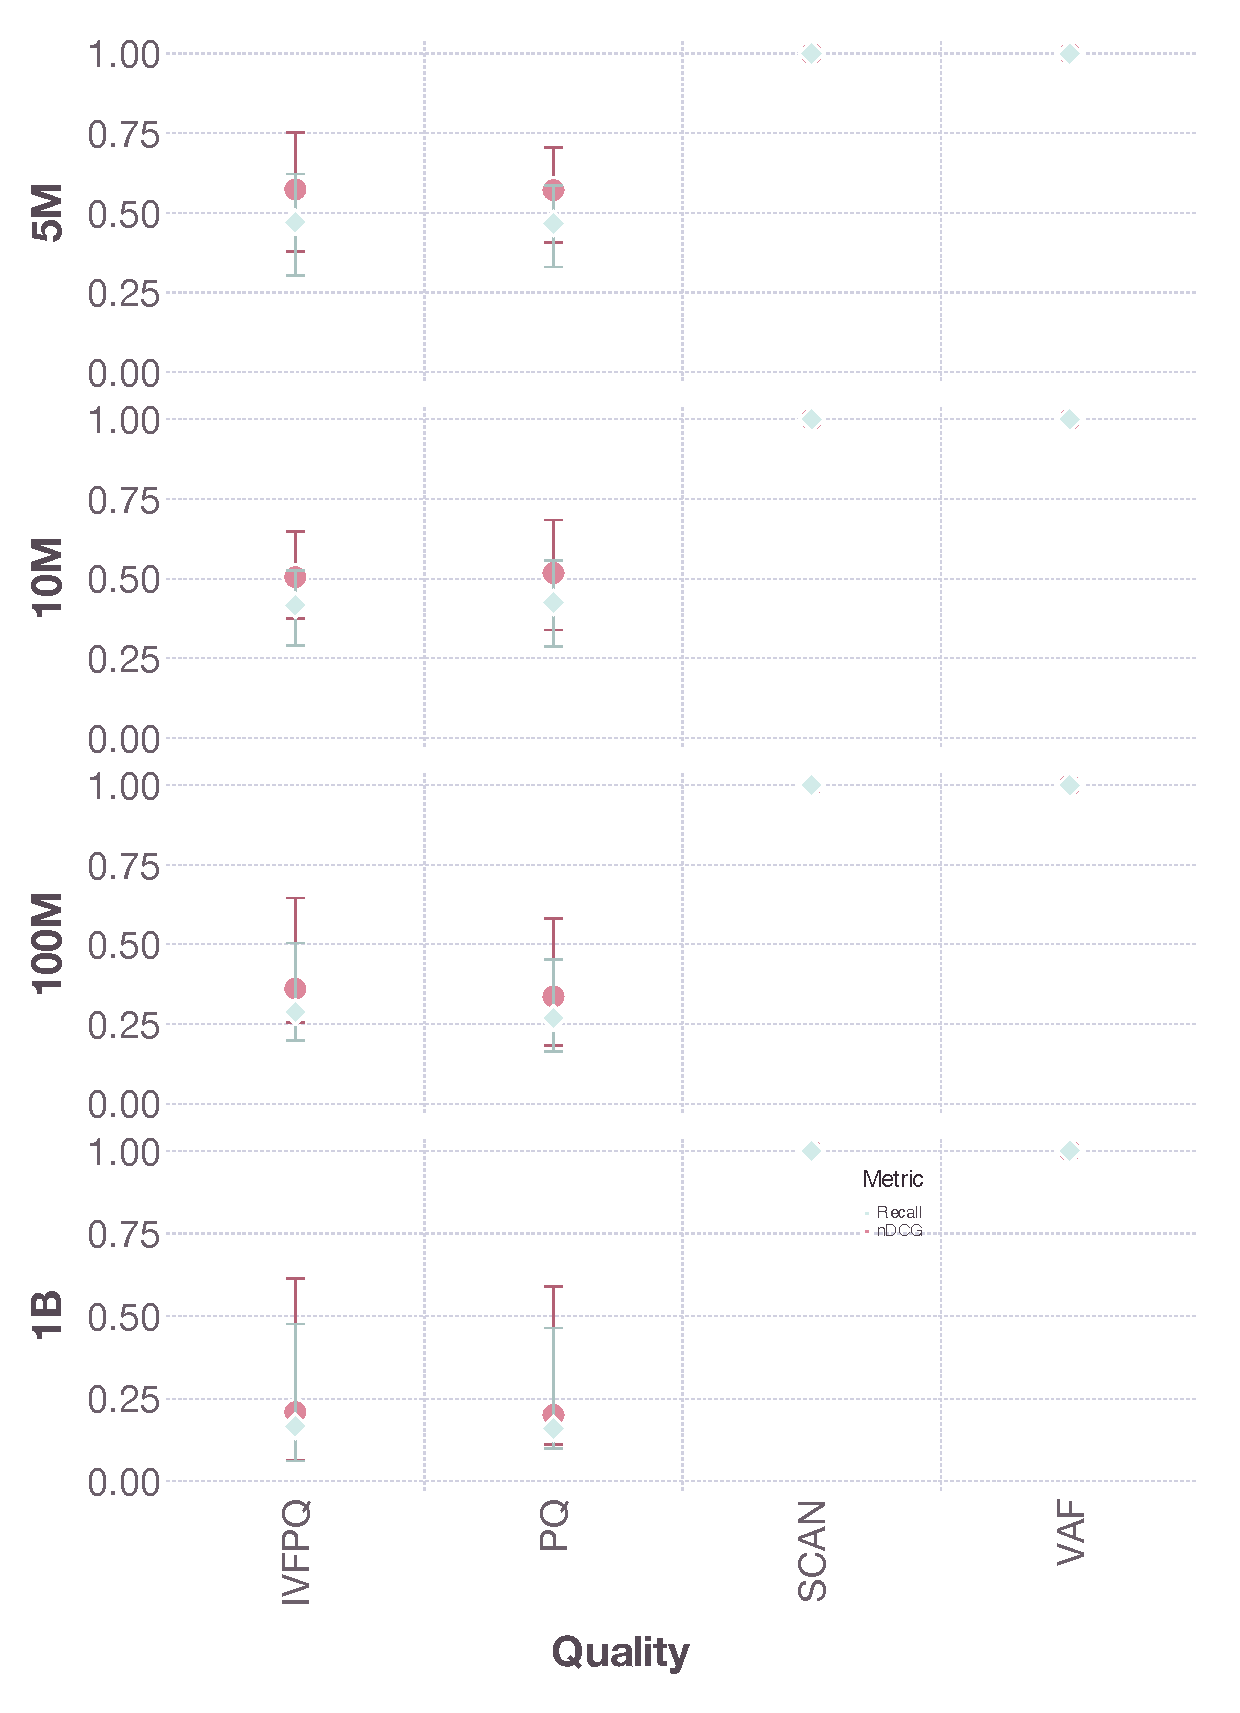
\includegraphics[width=\linewidth]{figures/bignns-cottontail-quality-Hybrid}
    \caption{Quality metrics for Cottontail DB during the hybrid query large-scale retrieval evaluation presented in \Cref{section:evaluation_bignns_cottontail}. Recall and \acrshort{dcg} are 1.0 for all execution strategies other than \acrshort{pq}, for which they exhibit rather low values with a large spread.}
    \label{figure:appendix_bignns_cottontail_hybrid_quality}
\end{figure}
